\chapter{Inspections, Tests, and Metrics}\hyperdef{part}{ivv}{}\label{ch:ivv}

\section{Inspection}\label{sec:inspect}
%%%%%%%%%%%%%%%%%%%%%%%%%%%%%%%%%%%%%%%%%%%%%%%%%%%%%%%%%%%%%%%%%%%%%%%%%%%%%%%%
% ivv_inspect.tex
% Inspections of the Simulation Interface Model
%
% 
%%%%%%%%%%%%%%%%%%%%%%%%%%%%%%%%%%%%%%%%%%%%%%%%%%%%%%%%%%%%%%%%%%%%%%%%%%%%%%%%

\inspection{Top-level Inspection}
\label{inspect:TLI}
This document structure, the code, and associated files have been inspected.
With the exception of the cyclomatic complexity of the
\verb|JeodTrickMemoryInterface::primitive attributes| method,
the \ModelDesc satisfies requirement~\traceref{reqt:toplevel}.
A waiver has been granted for this one exception.

\inspection{Design Inspection}
\label{inspect:design}
%\tracingall
Table~\ref{tab:design_inspection} summarizes the key elements of the
implementation of the \ModelDesc that satisfy requirements levied on the model.
By inspection, the \ModelDesc satisfies
requirements~\tracerefrange{reqt:hidden_data_visibility}{reqt:extensibility}.

\begin{longtable}%
  {||l @{\hspace{4pt}} %
   >{\raggedright\arraybackslash}p{1.38in} |%
   >{\raggedright\arraybackslash}p{3.95in}|}
\caption{Design Inspection}
\label{tab:design_inspection} \\[6pt]
\hline
\multicolumn{2}{||l|}{\bf Requirement} & \bf{Satisfaction}
\\ \hline\hline
\endfirsthead

\caption[]{Design Inspection (continued from previous page)} \\[6pt]
\hline
\multicolumn{2}{||l|}{\bf Requirement} & \bf{Satisfaction}
\\ \hline\hline
\endhead

\hline \multicolumn{3}{r}{{Continued on next page}} \\
\endfoot

\hline
\endlastfoot

\ref{reqt:hidden_data_visibility} & Hidden Data Visibility &
  The macro \verb|JEOD_MAKE_SIM_INTERFACES| provides the required
  simulation engine agnostic capability. The implementation of this macro
  is simulation engine specific. Trick-specific implementations make
  protected and private data visible to Trick.
\tabularnewline[4pt]

\ref{reqt:allocated_data_visibility} & Allocated Data Visibility &
  The member functions
  \verb|register_allocation| and \verb|deregister_allocation|
  in the abstract class \verb|JeodTrickMemoryInterface|
  specify the simulation engine agnostic capability. The implementations
  of these methods in the class \verb|JeodTrickMemoryInterface|
  make allocated data visible to Trick.
\tabularnewline[4pt]

\ref{reqt:sim_engine_interface} & Simulation Engine Interface &
  The only Trick dependencies outside of the \ModelDesc are the
  noted exception in the \DYNMANAGER. All other simulation engine
  interfaces are encapsulated within the \ModelDesc.
\tabularnewline[4pt]

\ref{reqt:integ_interface} & Integration Interface &
  The abstract class \verb|IntegratorInterface| provides the required
  simulation engine agnostic capabilities. Trick-specific
  classes that derive from this abstract class provide implementations
  of the required functionality in both the Trick 7 and Trick 10
  environments.
\tabularnewline[4pt]

\ref{reqt:job_cycle} & Job Cycle &
  The function \verb|JeodSimulationInterface::get_job_cycle|
  is the public interface to this required functionality.
  This invokes the pure virtual protected member function
  \verb|get_job_cycle_internal|.
  The class \verb|BasicJeodTrickSimInterface| implements this
  function in the context of a Trick-based simulation.
\tabularnewline[4pt]

\ref{reqt:trick_message_handler} & Trick Message Handler &
  The \ModelDesc provides the class \verb|TrickMessageHandler|, which
  derives from the class \verb|SuppressedCodeMessageHandler|
  and which implements the functionality required of a \verb|MessageHandler|
  using Trick's messaging system.
\tabularnewline[4pt]

\ref{reqt:checkpoint_restart} & Checkpoint/Restart &
  The \ModelDesc provides a generic checkpoint/restart capability in the
  form of classes that create and read from a sectioned checkpoint file.
  The class \verb|JeodTrick10MemoryInterface| uses these
  generic capabilities to provide the required ability to make
  JEOD-based simulations checkpointable and restartable in a
  Trick 10 environment.
\tabularnewline[4pt]

\ref{reqt:addr_name_xlate} & Address/Name Translation &
  The functions \verb|get_name_at_address| and \verb|get_address_at_name|
  in the classes \verb|JeodSimulationInterface| (static) and
  \verb|JeodMemoryInterface| (pure virtual)
  are the public interfaces to this required functionality.
  The class \verb|JeodTrickMemoryInterface| provides dummy
  implementations while \verb|JeodTrick10MemoryInterface| provides
  functional implementations of these functions.
\tabularnewline[4pt]

\ref{reqt:multiple_integ_groups} & Multiple Integration Groups &
  The \ModelDesc implements this requirement as a set of JEOD-agnostic
  classes (which may eventually be migrated out of JEOD) and the JEOD-aware
  class \verb|JeodDynbodyIntegrationLoop|.
\tabularnewline[4pt]

\ref{reqt:extensibility} & Extensibility &
  The \ModelDesc was carefully designed to have the public interfaces be in
  the form generic macros and abstract, simulation engine agnostic classes.
  The Trick independent demonstration and the test harness
  used in the JEOD unit tests illustrate to some extent
  that the model can be extended for use outside of the Trick environment.
\tabularnewline[4pt]

\end{longtable}


\section{Tests}
This section describes various tests conducted to verify and validate 
that the \ModelDesc satisfies the requirements levied against it.  
All verification and validation test source code, simulations and procedures 
are archived in the JEOD directory 
{\tt models/utils/integration/verif}.\relax

\test{Numerical Integration}\label{test:integ}
\begin{description}
\item[Background] The primary purpose of this test 
is to determine whether the \ModelDesc integration techniques
do indeed integrate states over time.
As every integration technique is subject to error, a secondary purpose of
this test is to assess the accuracy of the various integration techniques.

Several complicating factors arise when testing numerical propagation
techniques. Three such factors are
\begin{itemize}\vspace{-0.5\baselineskip}
\item Even the best numerical propagation will fail to provide accurate 
results when the characteristic frequency of the system being propagated 
approaches to the integration frequency.
\item Even the best numerical propagation will fail to provide accurate 
results when the integration frequency is much smaller than the 
characteristic frequency of the system being propagated.
\item Numerical errors tend to grow with time. With many integrators
this error growth is non-linear. Integrate for too long a time and the
result will be meaningless.
\end{itemize}
For a given problem, the integrated state will track the true state
to within a reasonable degree of accuracy
if the integration frequency is held to within some limited frequency range
and if the integration interval is not too long. This test characterizes
the various techniques supplied with JEOD to assess the integration
frequency and interval over which the techniques can be trusted.

\item[Test description] 
This test involves using the numerical integration techniques to propagate
five sample problems that have analytic solutions.
Three of these sample problems demonstrate the propagation of a body
rotating in three dimensional space
using quaternions as the generalized position
and angular velocities as the generalized velocity.
The other two sample problems demonstrate the propagation of a body
translating in three dimensional space, this time using Cartesian
position and velocity as the generalized position and velocity.
Note that these are the representations of rotational and translational state
used throughout in JEOD. The test articles are

\begin{description}
\item[A freely rotating (torque-free) spherical body] %
  A torque-free body with a spherical mass distribution has very simple
  dynamics. The body rotates at a constant angular rate about a fixed axis.

\item[A torque-free symmetric top] %
  Making the body have a single axis of symmetry adds the complicating
  factor of inertial torque. This fictitious torque is a consequence of
  using a non-inertial reference frame for the representation of rotational
  state.
  
\item[A simple rotational harmonic oscillator] %
  In this problem an external torque that is proportional to the angular
  displacement of the body from some reference orientation is applied to
  the body. The result is a simple harmonic oscillator.

\item[A body following a Keplerian orbit] %
  This is the first of the two translational state problems.
  In this problem the body is subject to a central inverse square
  force with the central object located at the origin of the integration
  frame. The result is a Keplerian orbit about the origin.
  The test harness for this problem can handle any closed orbit.
  Circular orbits are used in the tests below.

\item[A spring-mass-damper system]
  This final problem is that of a damped harmonic oscillator.
  The test harness can handle any kind of damping (under-damped,
  critically damped, and over-damped).
  A lightly damped oscillator is used in the tests below.  
\end{description}

In a sense these are overly simplistic problems, particular in their
canonical forms. The integration can be made a bit tougher by rotating
away from the canonical description. The test harness uses this
approach. This rotation from canonical adds a small amount of initial
error to the system.


This test involves Monte-Carlo testing over a wide range of integration 
frequencies and a large number of random initial conditions. 
Because of the large number of test cases involved
this test examines the behaviors of the various
integration techniques from a statistical point of view.
This test involves determining ``three-sigma'' error bounds as a function
of the sample problem, the integration technique, the integration frequency,
and the run duration. These assessments are made using order statistics.

Over a million test cases were produced to generate the results
described below.
Each run tests one set of the \{sample problem, integration technique,
integration frequency, run duration\} problem space.
The chosen integration technique is used to propagate
the dynamical equations of motion for the chosen sample problem,
with the integration occurring at the chosen frequency, and
the simulation running for the chosen amount of time.
Deviations between the propagated and computed states are
assessed during the course of the run, with
the worst-case deviation reported at the end of the run.

The integration frames for a given run are rotated from canonical by
pseudorandom amounts. This random variation was repeated 369 times (370 is
the minimum number of trials needed to assess the three-sigma bound
via interpolation on order statistics)
for each element of the problem space. After making the requisite number of
runs, order statistics were used to estimate the three-sigma error bounds.

\item[Test directory] {\tt SIM\_integ\_test} \\
The {\tt S\_define} uses the test scenario derivative and evaluation 
functions to propagate and integrate the selected states.
\item[Test scripts] {\tt run\_cases.pl} and {\tt scan\_runs.pl} \\
The first script runs the simulation many, many times. The second
script analyzes the output to estimate the three-sigma error bounds and
generates the plots displayed below.

\item[Success criteria] Any given integration technique will perform well
only for a limited span of time and only if the integration is performed
at some reasonable frequency. This presents a challenge in testing.
An overly strict set of criteria will result in all techniques deemed to
have failed. Instead, the performance is to be categorized as follows. 

The rotation test cases are deemed to perform
\begin{itemize}
\item Exceptionally if the three-sigma angular error bounds
  do not exceed $10^{-9}$ degrees,
\item Well if the three-sigma angular error bounds
  do not exceed $10^{-6}$ degrees,
\item Acceptably if the three-sigma angular error bounds
  do not exceed $10^{-3}$ degrees,
\item Marginally if the three-sigma angular error bounds
  do not exceed 1 degree, and
\item Unacceptably if the three-sigma angular error bounds
  exceed 1 degree.
\end{itemize}

The translation tests have similar error classifications:
\begin{itemize}
\item Exceptionally if the three-sigma relative position error bounds
  do not exceed $10^{-12}$,
\item Well if the three-sigma relative position error bounds
  do not exceed $10^{-9}$,
\item Acceptably if the three-sigma relative position error bounds
  do not exceed $10^{-6}$,
\item Marginally if the three-sigma relative position error bounds
  do not exceed $10^{-3}$, and
\item Unacceptably if the three-sigma relative position error bounds
  exceed $10^{-3}$.
\end{itemize}

\item[Test results]
The three-sigma error bounds are portrayed as log-log graphs in
figures~\ref{fig:ffsphere_err} to~\ref{fig:spring_damper_err}.

A synopsis of the results:
\begin{itemize}\vspace{-0.5\baselineskip}
\item Only the two fourth-order techniques, RK4 and ABM4, yield
exceptional performance. The optimal integration rate for these two
techniques is $\omega \Delta t \approx 0.05$ degrees for the investigated
non-stiff problems, or about 1 Hz for a vehicle in low Earth orbit.
\item None of the integration techniques perform exceptionally at 
very small ($\omega \Delta t < 10^{-4}$ degrees) time steps, which
is about 650 Hz for a vehicle in low Earth orbit.
\item All of the integration techniques break down as the 
integration frequency approaches the Nyquist frequency
($\omega \Delta t = 180$ degrees).
Where this breakdown occurs depends on the problem being solved and
on the integration technique being used to solve it.
All of the techniques provided with JEOD begin performing poorly
well below the Nyquist frequency.
\item Most of the integrators perform acceptably or better at some
intermediate integration frequency and for some limited amount of time.
The two marked exceptions are the Euler integrators.
The basic Euler technique fares quite poorly at all tested rates.
The symplectic Euler technique begins to perform marginally
(performance that might pass for acceptable accuracy in some circumstances)
at extremely fast integration frequencies.
\end{itemize}

In summary, basic Euler technique fails to meet any reasonable expectation
of accuracy requirements. The symplectic Euler technique performs marginally.
All of the other techniques meet accuracy requirements over a wide range
of integration frequencies. All of the techniques of course fail when the
integration frequency is too low. That failure is the nature of integrating
at a frequency too close to the Nyquist frequency.



\begin{figure}[hbtp]
\centering
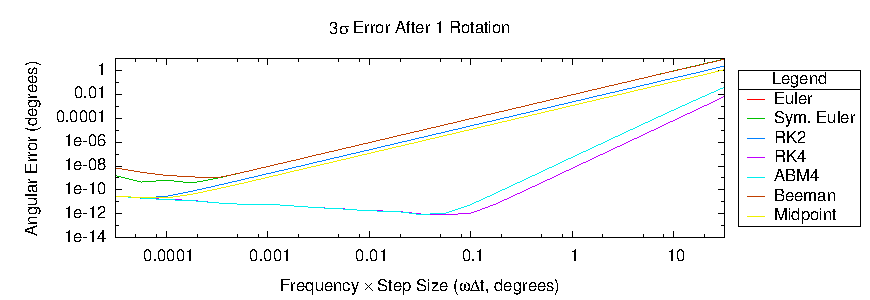
\includegraphics{figures/plot_RotationTestTorqueFreeSphere_revs_1_monte_err}
\vspace{2.0ex}
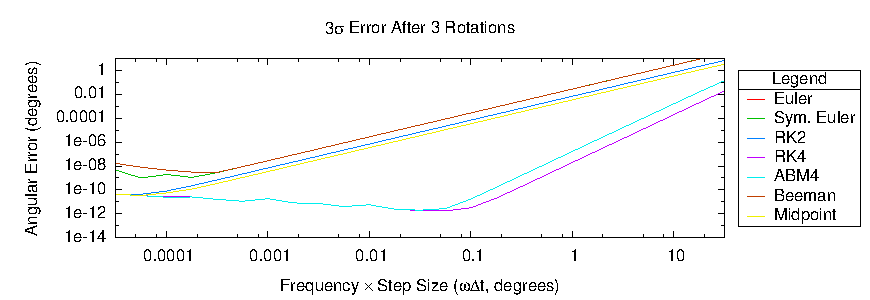
\includegraphics{figures/plot_RotationTestTorqueFreeSphere_revs_3_monte_err}
\vspace{2.0ex}
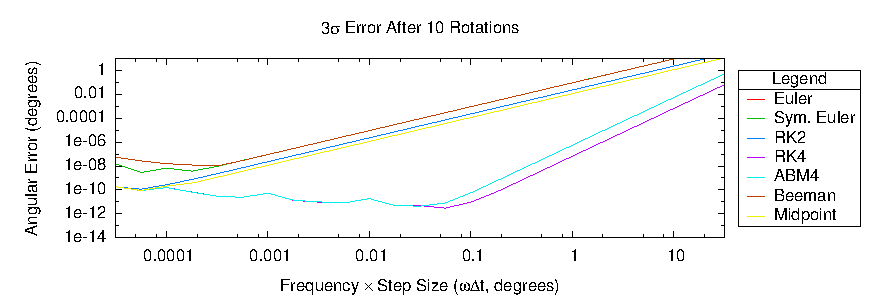
\includegraphics{figures/plot_RotationTestTorqueFreeSphere_revs_10_monte_err}
\vspace{2.0ex}
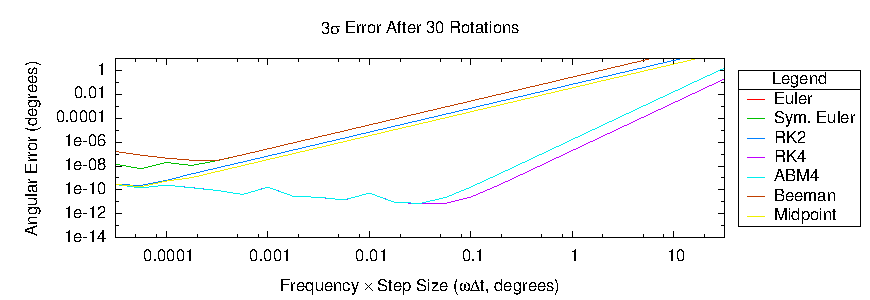
\includegraphics{figures/plot_RotationTestTorqueFreeSphere_revs_30_monte_err}
\caption{Torque-Free Sphere 3$\sigma$ Errors}
\label{fig:ffsphere_err}
\end{figure} 


\begin{figure}[hbtp]
\centering
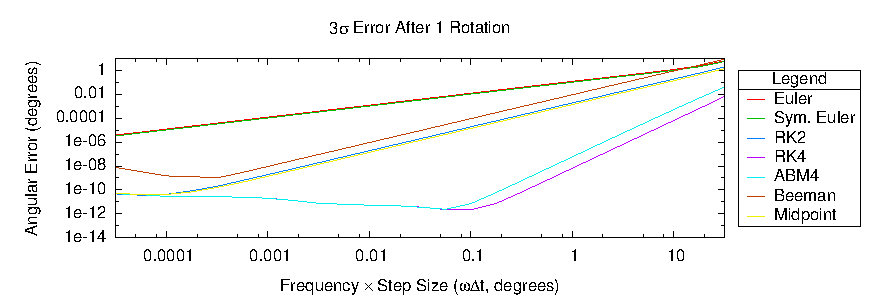
\includegraphics{figures/plot_RotationTestTorqueFreeSymTop_revs_1_monte_err}
\vspace{2.0ex}
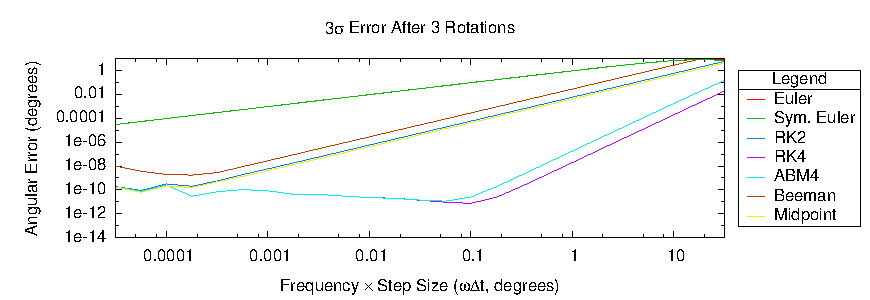
\includegraphics{figures/plot_RotationTestTorqueFreeSymTop_revs_3_monte_err}
\vspace{2.0ex}
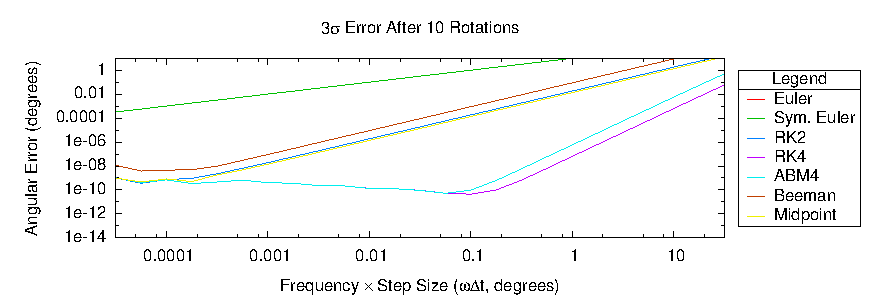
\includegraphics{figures/plot_RotationTestTorqueFreeSymTop_revs_10_monte_err}
\vspace{2.0ex}
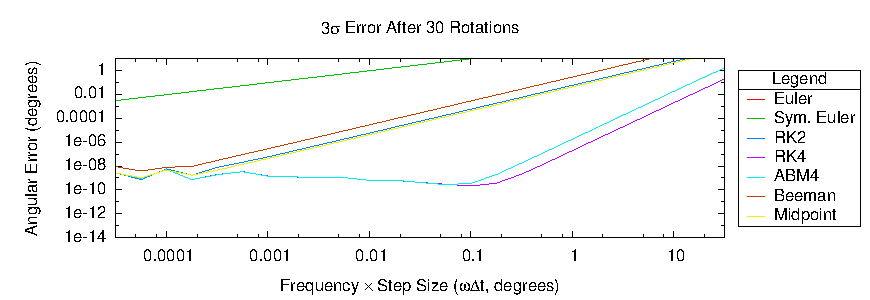
\includegraphics{figures/plot_RotationTestTorqueFreeSymTop_revs_30_monte_err}
\caption{Torque-Free Symmetric Top 3$\sigma$ Errors}
\label{fig:ffsymtop_err}
\end{figure} 

\begin{figure}[hbtp]
\centering
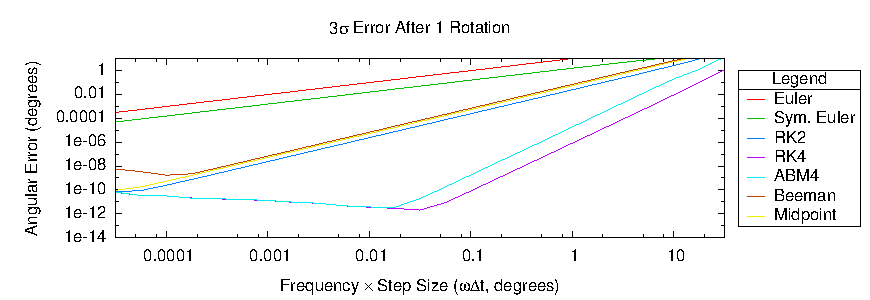
\includegraphics{figures/plot_RotationTestSHOSphere_revs_1_monte_err}
\vspace{2.0ex}
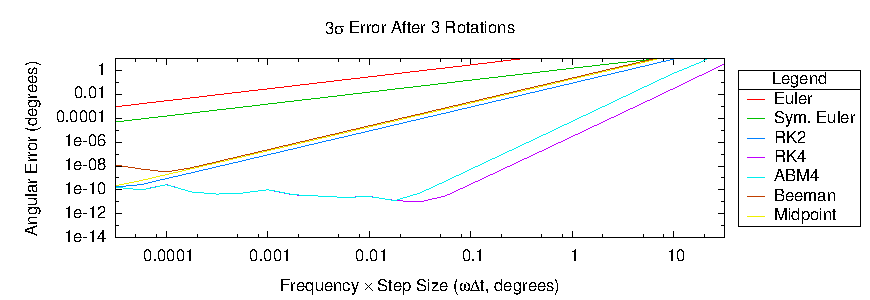
\includegraphics{figures/plot_RotationTestSHOSphere_revs_3_monte_err}
\vspace{2.0ex}
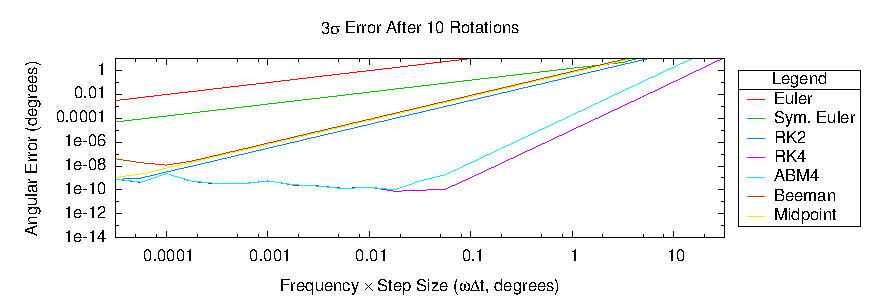
\includegraphics{figures/plot_RotationTestSHOSphere_revs_10_monte_err}
\vspace{2.0ex}
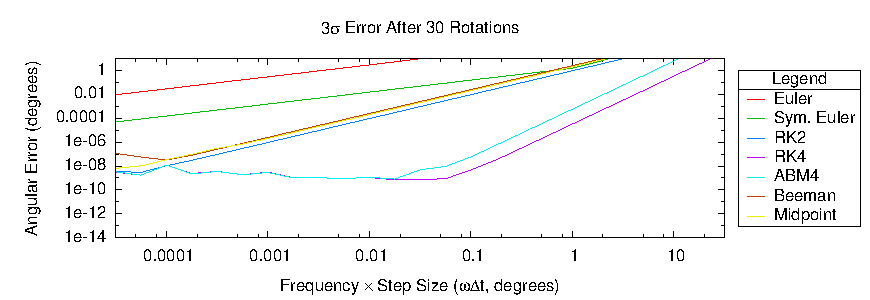
\includegraphics{figures/plot_RotationTestSHOSphere_revs_30_monte_err}
\caption{Spherical Harmonic Oscillator 3$\sigma$ Errors}
\label{fig:sho_sphere_err}
\end{figure} 

\begin{figure}[hbtp]
\centering
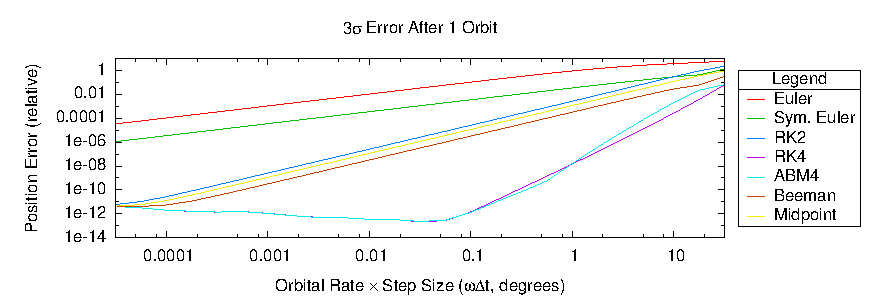
\includegraphics{figures/plot_TranslationTestOrbit_revs_1_monte_err}
\vspace{2.0ex}
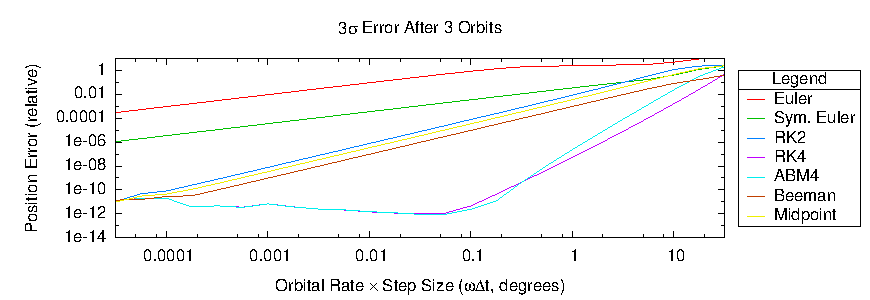
\includegraphics{figures/plot_TranslationTestOrbit_revs_3_monte_err}
\vspace{2.0ex}
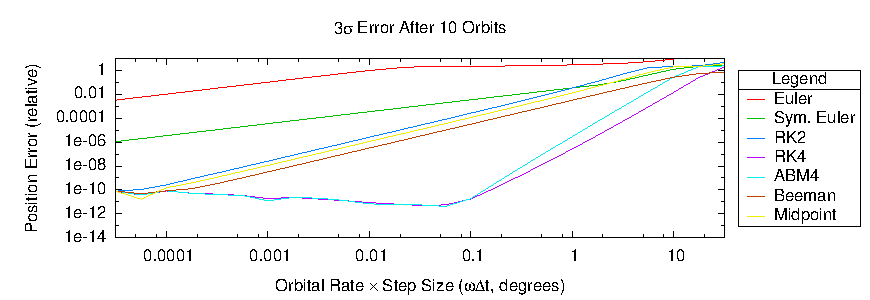
\includegraphics{figures/plot_TranslationTestOrbit_revs_10_monte_err}
\vspace{2.0ex}
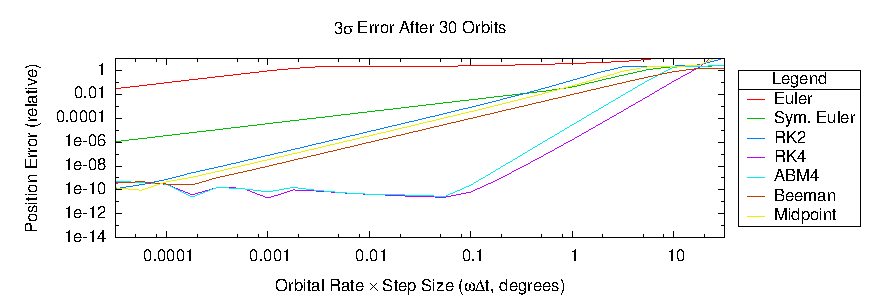
\includegraphics{figures/plot_TranslationTestOrbit_revs_30_monte_err}
\caption{Circular Orbit 3$\sigma$ Errors}
\label{fig:orbit_err}
\end{figure} 

\begin{figure}[hbtp]
\centering
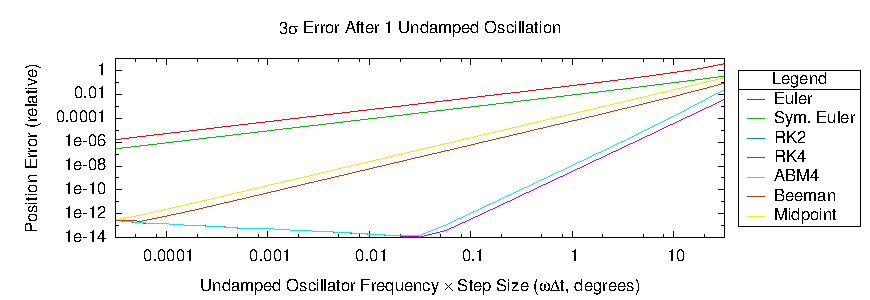
\includegraphics{figures/plot_TranslationTestSpringDamper_revs_1_monte_err}
\vspace{2.0ex}
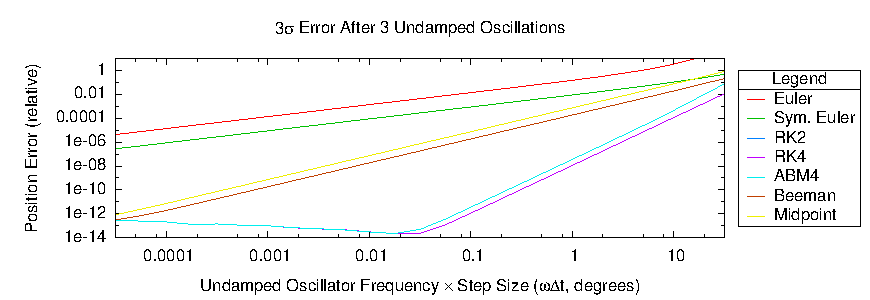
\includegraphics{figures/plot_TranslationTestSpringDamper_revs_3_monte_err}
\vspace{2.0ex}
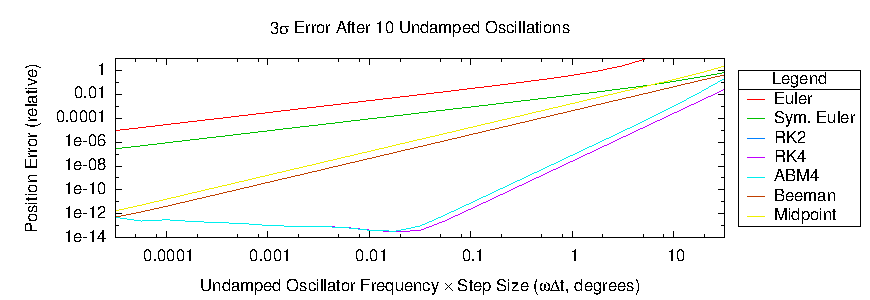
\includegraphics{figures/plot_TranslationTestSpringDamper_revs_10_monte_err}
\vspace{2.0ex}
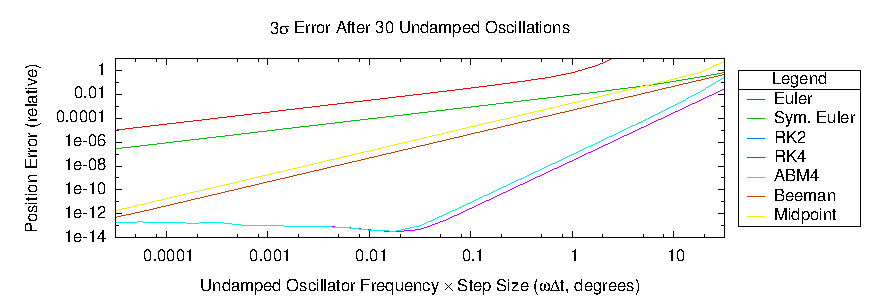
\includegraphics{figures/plot_TranslationTestSpringDamper_revs_30_monte_err}
\caption{Spring-Damper 3$\sigma$ Errors}
\label{fig:spring_damper_err}
\end{figure}


\item{Addendum to Test Results:}\ \newline
Comparison of the default configuration of the Gauss-Jackson method ($8^{th}$ 
order, no bootstrapping, no convergence testing) against the ABM4 and RK4 
methods was conducted for the orbit propagation test for a range of 
integration rates.

Preliminary results indicate:
\begin{itemize}
 \item \textbf{High rates} ($\omega \Delta t \sim O(10^-4 - 10^{-3}) deg.$): 
 \newline Surprisingly, the decrease in performance seen in ABM4 and RK4 is 
 not nearly so pronounced in Gauss-Jackson.  Consequently, Gauss-Jackson 
 showed marginally superior performance by one to two orders of magnitude 
 over 
 this range.  These tests were run over a 5-orbit period.
 \item \textbf{Mid-range rates} ($\omega \Delta t \sim O(10^-2 - 10^{-1}) 
 deg.$): 
 \newline Over this range, the performance stays flat, perhaps diminishing 
 slightly to be comparable to that of ABM4 and RK4.  These tests were run over 
 a 50-orbit period.
 \item \textbf{Low rates} ($\omega \Delta t\sim O(10^0 - 10^{1}) deg.$): 
 \newline
 The performance continues to diminish at longer time-steps, but much more 
 slowly than the ABM4 and RK4.  By $\omega \Delta t \approx 1 deg.$, the 
 Gauss-Jackson algorithm performs three to four orders of magnitude better 
 than the ABM4 and RK4 algorithms.  This trend continues until the ABM4 
 starts 
 to lose stability at around 10 degrees, at which point the Gauss-Jackson 
 performance falls to marginal.  By 30 degrees, RK4 has also lost stability, 
 and while Gauss-Jackson continues to propagate nicely, the accumulated 
 errors 
 are reaching around 10\% after 50 orbits.
\end{itemize}

The Gauss-Jackson algorithm has a number of user-definable parameters that 
control its behavior.  A description of these is found in the User Guide (see 
\textref{Gauss-Jackson 
Parameters}{sec:guide_simuser_gauss_jackson_parameters}), and verification of 
their functionality is found in Test~\ref{test:gauss_jackson}.

\item[Applicable Requirements]
This test completes the satisfaction of the
requirements~\traceref{reqt:use_er7_utils}
and~\traceref{reqt:supported_er7_techniques},
and partially satisfies the requirements 
~\traceref{reqt:extensibility}
and~\traceref{reqt:integration_problems}.

\end{description}
\clearpage


\test{Gauss-Jackson Parameters}\label{test:gauss_jackson}
\begin{description}
 \item [Background]
The Gauss-Jackson algorithm has a number of user-definable parameters that 
control its behavior.  A description of these is found in the User Guide (see 
\textref{Gauss-Jackson 
Parameters}{sec:guide_simuser_gauss_jackson_parameters}).  This test verifies 
their functionality, and provides a quantitative assessment of their 
respective behaviors for propagation in the very simple case of a circular 
orbit in a spherical gravity field.

\item [Test directory] {\tt SIM\_GJ\_test} \\

\item[Test description]
A number of runs were made to perform the following tests:
\begin{enumerate}
 \item A comparison of Gauss-Jackson against RK4 for a range of time-steps.
 \item A study of the effect of adding the evaluation-step after the 
 corrector-step, and altering the convergence threshold.
 \item A study of the effect of adding the bootstrap method, for both short 
 time-step and long time-step simulations.
 \item A study of the extent to which the order of the integrator affects its 
 accuracy. 
\end{enumerate}

All runs were performed on a very simple orbital case, involving a vehicle in 
a circular orbit, of period around 7000 seconds, around an earth-like planet 
with spherical gravity.  The only comparison investigated was the magnitude of 
the position vector against the reference orbital radius.
The simplicity of this test must be considered when 
evaluating the results presented here; the validity of applying these data to 
more complex environments is inherently questionable.  Nevertheless, these 
data provide a starting point for identifying optimal integrator 
configuration.

\item[Success criteria]
The fundamental test is to ensure that the simulation will run with a diverse 
array of integrator parameters.  The secondary test is to quantify the effect 
of changing those parameters.

\item[Test results]
The fundamental test passes, there was no configuration found for which the 
simulation failed.

The quantitative comparison of the different parameters follows.

\item[Gauss-Jackson versus RK4]\ \newline
The Gauss-Jackson integrator used to compare against RK4 uses the default 
configuration - $8^{th}$ order, no evaluation step, no bootstrapping.  
Integration step sizes are tested in powers of 10; in 
Figure~\ref{fig:GJ_RK_logs}, the legend indicates the step-size:
\begin{itemize}
 \item step00 - 0.01 seconds
 \item step0 - 0.1 seconds
 \item step1 - 1 second
 \item step10 - 10 seconds
 \item step 100 - 100 seconds
\end{itemize}

\begin{figure}[!ht]
\centering
\includegraphics[width=3.5in]{figures/GJ_RK_logs.jpg}
\caption[Variation with Time of Orbital Position Error]{The variation with time of the log of the averaged (over the 
simulation to time, t) absolute value of the relative difference between the 
magnitude of the numerically integrated position vector and the radius of the 
circular orbit that the vehicle follows; $log_{10} (<\frac{|\vec{r}| - 
r_{circ}}{r_{circ}}>) \sim t$.   Data are taken from Gauss-Jackson and RK4 
integrators with a selection of integration rates.}
\label{fig:GJ_RK_logs}
\end{figure}

Three runs stand out as being particularly weak.  As expected, the RK4 
algorithm performs poorly at 10-second and 100-second cycle-times 
(corresponding to $\omega \Delta t \sim 0.5, 5 deg$).  The 
Gauss-Jackson algorithm also 
struggles at the 100-second step, but this is not particularly surprising 
since it 
is initialized with a RK4 integrator running at 100 seconds.  See the 
bootstrapping comparison below for details on circumventing this problem.

Of the remaining runs, the two algorithms running at 0.01 seconds fare 
relatively poorly.  These five runs are removed for comparison of the 
variation with time of the position error, $\frac{|\vec{r}| - 
r_{circ}}{r_{circ}}$ (where $r_{circ}$ is the reference orbital radius), shown in 
Figure~\ref{fig:GJ_RK_performance}.

\begin{figure}[!ht]
\centering
\includegraphics[width=3.5in]{figures/GJ_RK_performance.jpg}
\caption[Variation with Time of Orbital Position Error]{The variation with 
time of the 
relative difference between the 
magnitude of the numerically integrated position vector and the radius of the 
circular orbit that the vehicle follows; $\frac{|\vec{r}| - 
r_{circ}}{r_{circ}} \sim t$.  Data are taken from Gauss-Jackson and RK4 
integrators with a selection of integration rates.}
\label{fig:GJ_RK_performance}
\end{figure}

The results indicate limited differential between the algorithms at the 
time-steps selected for Figure~\ref{fig:GJ_RK_performance}, i.e., 0.1 seconds 
to 1.0 seconds for RK4; 0.1 seconds to 10.0 seconds 
for GJ.

\item[Significance of the Evaluate Step in Predict-Correct-Evaluate]\ 
\newline
For this illustration, baseline GJ integrators ($8^{th}$ order, no evaluation 
step, no bootstrapping) with 1-second and 100-second integration steps were 
compared against similar GJ integrators with a convergence criterion applied 
to them, specifying that the state must converge to within 1 part in 
$10^{15}$, approximately the limit of the \textit{double} data specification. 
Such a tight requirement was imposed because of the simplicity and 
predictability of the simulation; the integrator should be able to get very 
close to the converged solution with only one correction phase.

Indeed, even with such a tight requirement, there was no discernible 
difference in the results from the 1-second integrators.  At the 100-second 
integration rate, a very small difference (about 1 part in $10^4$) was 
observed by the end of the simulation in the value $\frac{|\vec{r}| - 
r_{circ}}{r_{circ}}$.  With the value $\frac{|\vec{r}| - 
r_{circ}}{r_{circ}} \sim O(10^{-7})$, this indicates a difference in the 
magnitude of the 
position, resulting from the performance of the evaluate step, of about 1 part 
in $10^{11}$.

\item[Effect of Adding the Bootstrap Method]\ \newline 
The bootstrap method takes a specified value for the maximum RK4 time-step 
that can be used in the GJ integrator priming phase, and gradually ramps that 
time-step up until the GJ integrator is running 
with a cycle-time equal to the desired tour time.  The bootstrap method 
should be most useful when the GJ tour time is in the regime where RK4 
performs poorly.

First, an erroneous application was tested to ensure that mis-application
does not cause undesirable behavior.  The 1-second integrator was 
bootstrapped with a 
0.1-second RK4 integrator, and then with a 0.01-second RK4 integrator (note 
that at 1-second, RK4 is near its optimal performance, so bootstrapping is 
not needed in this scenario, and bootstrapping with a sub-optimal time-step 
is clearly a detrimental process).  As shown in 
Figures~\ref{fig:GJ_bootstrap_short_log}
and ~\ref{fig:GJ_bootstrap_short_val}, the effect in this regime is minimal; 
indeed the 
non-bootstrapped simulation is indistinguishable from the one bootstrapped at 
0.1-seconds;  both of these marginally outperform the third simulation.

\begin{figure}[!ht]
\centering
\includegraphics[width=3.5in]{figures/GJ_bootstrap_short_log.jpg}
\caption[Variation with Time of Orbital Position Error]
{The variation with time of the log of the averaged (over the 
simulation to time, t) absolute value of the relative difference between the 
magnitude of the numerically integrated position vector and the radius of the 
circular orbit that the vehicle follows; $log_{10} (<\frac{|\vec{r}| - 
r_{circ}}{r_{circ}}>) \sim t$.  Data are taken from Gauss-Jackson 
integrators with 1-second rates, with and without bootstrapping.}
\label{fig:GJ_bootstrap_short_log}
\end{figure}


\begin{figure}[!ht]
\centering
\includegraphics[width=3.5in]{figures/GJ_bootstrap_short_val.jpg}
\caption[Variation with Time of Orbital Position Error]
{The variation with 
time of the 
relative difference between the 
magnitude of the numerically integrated position vector and the radius of the 
circular orbit that the vehicle follows; $\frac{|\vec{r}| - 
r_{circ}}{r_{circ}} \sim t$.  Data are taken from Gauss-Jackson integrators 
with 1-second rates, with and without bootstrapping.}
\label{fig:GJ_bootstrap_short_val}
\end{figure}

Next, the correct application of the bootstrap was evaluated, bootstrapping 
the 100-second integrator off a 1-second (i.e. near-optimal) RK4 priming 
integrator.  The effect is quite 
pronounced, producing an improvement of around 5 orders of magnitude, shown in
Figure~\ref{fig:GJ_bootstrap_long_log}.  This improvement makes the 
100-second GJ integrator a reasonable tool, still slightly off-optimal for 
numerical precision, but with significantly improved speed in the situation 
where the environment takes significant computation.
(Note - a period of 100-seconds corresponds to an angular period of 
approximately 5 degrees).

Further testing indicates that, while the bootstrap algorithm significantly 
enhances performance, it is insufficient to overcome the rapid degradation of 
performance for angular rates greater than about 5 degrees per step.  As 
illustrative points, at 15 degrees the performance is back to the $10^{-7}$ 
range that we had a 5-degrees without bootstrapping; by 30 degrees, the 
performance is worse, even with bootstrapping, than that of RK4 at 5-degrees; 
by 40 degrees, the algorithm becomes completely unreliable.

\begin{figure}[!ht]
\centering
\includegraphics[width=3.5in]{figures/GJ_bootstrap_long_log.jpg}
\caption[Variation with Time of Orbital Position Error]
{The variation with time of the log of the averaged (over the 
simulation to time, t) absolute value of the relative difference between the 
magnitude of the numerically integrated position vector and the radius of the 
circular orbit that the vehicle follows; $log_{10} (<\frac{|\vec{r}| - 
r_{circ}}{r_{circ}}>) \sim t$.  Data are taken from Gauss-Jackson 
integrators with 100-second rates, with and without bootstrapping.}
\label{fig:GJ_bootstrap_long_log}
\end{figure}
\clearpage

\item[Effect of Changing the Order of the Integrator]\ \newline
For such a simple scenario, it is not expected that the order of the 
integrator should have a significant effect, and that is what is found.  
Figure~\ref{fig:GJ_order_short_log} illustrates the performance for 
integrators with order 2, 4, 8, 12, and 16.  While the $16^{th}$ order 
provides the best performance, it is a marginal result, and is followed by 
the $2^{nd}$ order.  No conclusion can be drawn about the effect of changing 
the order of the integrator from this scenario.

\begin{figure}[!ht]
\centering
\includegraphics[width=3.5in]{figures/GJ_order_short.jpg}
\caption[Variation with Time of Orbital Position Error]
{The variation with time of the log of the averaged (over the 
simulation to time, t) absolute value of the relative difference between the 
magnitude of the numerically integrated position vector and the radius of the 
circular orbit that the vehicle follows; $log_{10} (<\frac{|\vec{r}| - 
r_{circ}}{r_{circ}}>) \sim t$.  Data are taken from Gauss-Jackson 
integrators with 1-second rates, with varying order.}
\label{fig:GJ_order_short_log}
\end{figure}

\item[Applicable Requirements]
This test completes the satisfaction of requirements
\traceref{reqt:long_arc_integration}
and~\traceref{reqt:integration_problems}.

\end{description}

\clearpage

\test{Multiple Integrators}\label{test:multiple_integrators}
\begin{description}
\item[Background]
The purpose of this test is to verify that the model can accommodate
an arbitrary number of state integrators. The ability of the \ModelDesc to
accommodate multiple integrators was implicitly demonstrated in
test~\ref{test:integ}. The large number of individual test cases needed by that
test made it highly advantageous to instrument the test harness code with
the ability to test multiple integrators in parallel. This test explicitly
demonstrates that capability.

\item[Test directory] {\tt SIM\_integ\_test} \\
The same simulation is used for all of the \ModelDesc verification tests.

\item[Test scripts] {\tt run\_cases.pl} and {\tt test\_multi.tcsh} \\
The latter script drives the former script, which is the same script
used to drive the simulation for test~\ref{test:integ}.

\item[Test description]
The {\tt test\_multi.tcsh} script is used to generate what should be two
identical sets of output data. The script is used to run the simulation a 
number
of times in series for one set (N simulation runs of one case each) and in
parallel for the other set (one simulation run of N test cases). The test is
repeated for each integration technique provided by JEOD.

\item[Success criteria]
A test of an individual technique succeeds if the serial and parallel runs
generate identical output. The test succeeds as a whole if each of the 
individual tests succeed.

\item[Test results]
All tests pass.

\item[Applicable Requirements]
This test partially satisfies requirements
~\traceref{reqt:multiple_states}
and~\traceref{reqt:multiple_integrators}.

\end{description}


\test{Model Extensibility}\label{test:extensibility}
\begin{description}
\item[Background]
The purpose of this test is to assess whether a numerical integration
technique that is not supported by JEOD can be created and used in
a simulation.
\item[Test description] The second order midpoint method is not supported
in JEOD. This test involves implementing this method as a demonstration
of the extensibility of the model.
\item[Success criteria]
The test succeeds if the method can be implemented within the confines
of the \ModelDesc architecture and successfully used in lieu of the
supported methods in the various tests of algorithm accuracy.
\item[Test results]
The new integration model was successfully implemented and tested.
The results from using this integration technique are presented
in test~\ref{test:integ}.
\item[Applicable Requirements]
This test completes the satisfaction of 
requirement~\traceref{reqt:extensibility}.

\end{description}


\test{Multiple Integration Groups}\label{test:multiple_groups}
\begin{description}
 \item[Background]
 The purpose of this test is to verify that a simulation can operate with  
 multiple integrators operating simultaneously with different conditions. 
 \item [Test Description] The simulation SIM\_prop\_planet\_T10 utilizes two 
 different integration rates for propagation of planets (propagating their 
 state, rather than using the ephemeris model).  At one point in the 
 simulation, one of the bodies is switched from one integration group to the 
 other.
 \item [Success Criteria]
 The simulation needs to demonstrate:
 \begin{enumerate}
  \item Both groups can propagate independently at different rates.
  \item A body can successfuly transition from one group to the other.
 \end{enumerate}
 \item [Test Results]  Both test criteria were satisfied.
 \item[Applicable Requirements]
This test completes the satisfaction of 
requirements~\traceref{reqt:multiple_states}
and~\traceref{reqt:multiple_integrators}.

\end{description}


\section{Regression Tests}
Only the Gauss-Jackson test \textit{SIM\_GJ\_test} is in a form that is 
suitable for regression testing.

The other tests use input files that are created in temporary directories
and deleted after use. None of these tests use logged data.

Several regression tests were created to address this issue. The
regression tests are not used to verify and validate the model.
They are used instead to determine whether something went awry
during nightly builds and prior to release. The regression tests
follow the standard JEOD naming convention, with input files in subdirectories
within the SET\_test directory and comparison data in in corresponding
subdirectories in the SET\_test\_val directory.


\newpage
\boilerplatetraceability

\newpage
\boilerplatemetrics


%\section{Metrics}
%
%
%
%Table~\ref{tab:coarse_metrics} presents coarse metrics on the source
%files that comprise the model.
%
%\input{coarse_metrics}
%
%Table~\ref{tab:metrix_metrics} presents the cyclomatic complexity of the 
%methods defined in the model.
%
%\input{metrix_metrics}
%
%\newpage
%\section{Requirements Traceability}
%
%Table~\ref{tab:reqt_ivv_xref} summarizes the inspections and tests
%that demonstrate the satisfaction of the requirements levied on the model.
%
%\begin{table}[htp]
%\centering
%\caption{Requirements Traceability}
%\label{tab:reqt_ivv_xref}
%\vspace{1ex}
%\begin{minipage}{\textwidth}
%\centering
%\begin{tabular}{||l @{\hspace{4pt}} l|l @{\hspace{2pt}} l @{\hspace{4pt}} l|} 
%\hline
%\multicolumn{2}{||l|}{\bf Requirement} &
%\multicolumn{3}{l|}{\bf Inspection or test} \\ \hline\hline
%\ref{reqt:toplevel} & Project Requirements &
%     Insp. & \ref{inspect:TLI}     & Top-level Inspection
%\tabularnewline[4pt]
%\ref{reqt:supported_techniques} & Supported Techniques &
%     Insp. & \ref{inspect:math} & Mathematical Formulation \\
%  && Test  & \ref{test:integ}   & Numerical Integration
%\tabularnewline[4pt]
%\ref{reqt:extensibility} & Extensibility &
%     Insp. & \ref{inspect:design} & Design Inspection \\ 
%  && Test  & \ref{test:integ}     & Numerical Integration
%\tabularnewline[4pt]
%\ref{reqt:state_integration} & State Integration &
%     Insp. & \ref{inspect:design} & Design Inspection \\ 
%  && Test  & \ref{test:integ}     & Numerical Integration \\
%  && Test  & \ref{test:behavior}  & Behavior Test
%\tabularnewline[4pt]
%\ref{reqt:multiple_states} & Multiple States &
%     Insp. & \ref{inspect:design} & Design Inspection \\ 
%  && Test  & \ref{test:multiple}  & Multiple Integrators
%\tabularnewline[4pt]
%\ref{reqt:time_propagation} & Time Propagation &
%     Insp. & \ref{inspect:design} & Design Inspection \\
%  && Test  & \ref{test:behavior}  & Behavior Test
%\tabularnewline[4pt]
%\ref{reqt:integrator_constructor} & Integrator Construction &
%     Insp. & \ref{inspect:design} & Design Inspection \\ 
%  && Test  & \ref{test:integ}     & Numerical Integration
%    \footnote{Tests~\ref{test:integ} and~\ref{test:multiple} would not
%    work correctly if the integrator constructor factory did not properly
%    create integrator constructors or if the integrator constructors did
%    not create time and state integrators of the same type.
%    \label{fn:integrator_constructor_repeat}} \\
%  && Test  & \ref{test:multiple}  & Multiple Integrators
%     \footref{fn:integrator_constructor_repeat} \\
%  && Test  & \ref{test:behavior}  & Behavior Test
%    \footnote{The behavior test explicitly shows which integrator constructor
%    is in use and which time and state integrators are created by the
%    integrator constructor.}
%\tabularnewline[4pt]
%\ref{reqt:no_leaks} & Memory Management &
%     Insp. & \ref{inspect:memory} & Memory \\
%  && Test  & \ref{test:behavior}  & Memory Test
%\tabularnewline[4pt]
%\hline
%\end{tabular}
%\end{minipage}
%\end{table}
